\subsection{Desarrollo de la funcionalidades básicas}
\label{sec:desarrollo_funcionalidades_basicas}

En esta sección se describe el proceso de implementación de las funcionalidades básicas de la aplicación OTT. Como 
se indicó en secciones anteriores, las tecnologías principales utilizadas para el desarrollo son JavaScript, HTML y CSS, 
que permiten crear una interfaz interactiva, dinámica y adaptable a diferentes dispositivos y plataformas.

\subsubsection{Indicaciones previas}
\label{sec:indicaciones_previas}

Esta sección describe el comportamiento básico de la aplicación cuando se utiliza en televisores, ya que este es el enfoque principal y ha supuesto 
los mayores desafíos durante el desarrollo del código.

El desarrollo para televisores presenta una particularidad: la aplicación debe estar diseñada para ser controlada con un mando a distancia. Aunque 
algunas televisiones ofrecen la opción de utilizar un "magic remote", un mando que incluye un puntero que se mueve por la pantalla, muchos modelos no cuentan 
con esta funcionalidad. Desarrollar la aplicación solo para este tipo de dispositivos limitaría significativamente el mercado. Por ello, la aplicación 
ha sido diseñada desde un enfoque que permite su uso con un mando tradicional.

Aun así, también se ha contemplado la posibilidad de que la aplicación sea compatible con un puntero o ratón, como en el caso de los ordenadores, 
dado que, aunque este no fue un objetivo en las primeras versiones, uno de los principales propósitos del código es ser transversal y adaptable a 
cualquier dispositivo.

\subsubsection{Creación de los componentes de la aplicación}
\label{sec:creacion_componentes_aplicacion}

El primer paso del desarrollo fue la creación de la estructura básica de la aplicación y de los primeros componentes, sobre los cuales se ejecutan 
las funcionalidades principales. Estos componentes incluyen los menús, los "widgets" y los contenidos.

La creación de estos componentes sigue un enfoque en cascada. Cuando se inicia la aplicación, se realiza una llamada a la API de la empresa para obtener 
un archivo JSON conocido como "interfaz". Este JSON contiene la información principal para configurar la aplicación, incluyendo los colores (fondo, botones, 
textos), fuentes, textos legales, imágenes (logos, splash, etc.), y otros elementos utilizados para la personalización del cliente. Además, este archivo 
también proporciona la información sobre los menús que estarán disponibles en la aplicación.

Para la creación de los menús, existen dos opciones: menús con una pantalla asignada o menús con un comportamiento predefinido. Los menús con comportamiento 
predefinido incluyen el menú de configuración, búsqueda y catálogo, que no requieren información específica sobre la pantalla que deben mostrar.

\begin{itemize}
    \item \textbf{Configuración:} Este menú aloja las distintas opciones de configuración de la aplicación. Según las características de la aplicación, 
    se mostrarán diferentes opciones. Por ejemplo, si la aplicación admite múltiples idiomas, en este menú se podrá cambiar el idioma. Si hay usuarios 
    registrados, se mostrará la información del usuario y se podrá cerrar sesión. Una funcionalidad común a todas las aplicaciones es la opción de mostrar 
    los términos y condiciones.
    
    \item \textbf{Búsqueda:} Este menú permite filtrar todos los contenidos de la aplicación por el nombre del contenido, proporcionando una funcionalidad de búsqueda.
    
    \item \textbf{Catálogo:} También conocido como "A la carta", muestra en una sola página todos los contenidos disponibles en la aplicación.
\end{itemize}

En el caso de los menús que tienen una pantalla asignada, esta contiene la lista de "widgets" que deben mostrarse. Los "widgets" son contenedores de 
elementos, y según su tipo, tendrán un diseño y unas funcionalidades asignadas. Además, para cada widget existirá una lista de contenidos junto con 
la información de cada uno de ellos. 

Por lo tanto, la creación de las pantallas principales se realiza de la siguiente manera:

\begin{itemize}
    \item Se obtiene la información del menú a través de la API.
    \item Se analiza para determinar si es un menú predefinido o si tiene una pantalla asignada. 
    \begin{itemize}
        \item Si es un menú predefinido, se crea la pantalla según el comportamiento predefinido.
        \item Si tiene una pantalla asignada, se obtiene la información de la pantalla. 
        \begin{itemize}
            \item Se crea el elemento del DOM que contendrá la pantalla.
            \item A partir de la lista de widgets, se crea un elemento del DOM para cada uno de ellos.
            \item Se obtiene la información de los contenidos de cada widget.
            \item Se crea cada uno de los contenidos con las características correspondientes, en función del tipo de widget que los contiene.
            \item Se añade cada contenido al widget correspondiente en el orden adecuado.
            \item Se añade el widget al elemento del DOM que contiene la pantalla.
        \end{itemize}
    \end{itemize}
\end{itemize}

Durante la creación de cada elemento HTML, se le asignan una serie de clases según el tipo de elemento y widget correspondiente. Estas clases permiten 
aplicar el estilo a través de las hojas de estilo CSS.

El tipo de widget también determina el comportamiento de los contenidos que contiene. Por ejemplo, si el widget es de tipo \textit{featured} con el campo 
\textit{slider} activado, los contenidos destacados se mostrarán en un carrusel. Si el widget es de tipo \textit{mosaico}, los contenidos se mostrarán en 
una cuadrícula, y el movimiento, en lugar de ser una lista que se desplaza horizontalmente, será una cuadrícula que se mueve en ambas direcciones.


\subsubsection{Movimiento por la aplicación}
\label{sec:movimiento_aplicacion}
Una vez creados los elementos de la aplicación, el siguiente paso es habilitar la navegación dentro de ella. Para ello, se ha creado una serie de funciones 
que permiten moverse por los distintos elementos de la aplicación. Se ha tenido en cuenta que la aplicación será utilizada con un mando a distancia, 
por lo que el movimiento debe ser gestionado y controlado por el código.

Al utilizar la aplicación en televisores, es fundamental que exista un foco en un elemento en todo momento. Este foco indica en qué parte de la aplicación 
se encuentra el usuario y permite la navegación. En las pantallas principales de esta aplicación, se ha utilizado un foco fijo, es decir, el foco permanece 
en la misma posición casi siempre y los elementos se mueven en función de la dirección en la que el usuario navegue.

El movimiento a través de los widgets se realiza de la siguiente manera:

\begin{itemize}
    \item \textbf{Movimiento horizontal:} Utilizando las teclas de dirección izquierda y derecha. Si el usuario se encuentra en un widget, el movimiento 
    se realizará sobre los contenidos de dicho widget. Al pulsar una tecla de dirección, el widget se desplaza horizontalmente en la dirección indicada, 
    colocando el elemento seleccionado en la posición del foco.
    
    \item \textbf{Movimiento vertical:} Se realiza con las teclas de dirección arriba y abajo. Si existen widgets adicionales en la dirección pulsada, 
    la pantalla se desplazará hacia arriba o hacia abajo hasta colocar el elemento seleccionado en la posición del foco.
    
    \item \textbf{Movimiento en carrusel:} En caso de que el widget sea de tipo \textit{featured} con el campo \textit{slider} activado, el movimiento 
    se realiza dentro del carrusel de contenidos destacados. El desplazamiento horizontal cambia la imagen y la información mostrada en el carrusel.
    
    \item \textbf{Movimiento en mosaico:} Para los widgets de tipo \textit{mosaico}, el movimiento se realiza dentro de una cuadrícula de contenidos. 
    Los elementos se ordenan en filas de izquierda a derecha y de arriba hacia abajo. El movimiento vertical desplaza la pantalla hacia arriba o hacia abajo, 
    mientras que el horizontal mueve el foco hacia el contenido seleccionado.
\end{itemize}

El movimiento por el menú lateral es más sencillo. Se puede acceder al menú pulsando el botón \textit{return} desde cualquier pantalla principal, 
o bien pulsando la tecla de dirección izquierda si no quedan más elementos a la izquierda. Una vez seleccionado el menú, este se despliega, mostrando 
tanto los iconos como los nombres de los menús. El usuario puede moverse por el menú con las teclas de dirección arriba y abajo, destacando el 
elemento seleccionado con un aumento de tamaño.


\begin{figure}[H]
    \centering
    \begin{subfigure}[c]{0.1\textwidth} 
        
\includegraphics[width=\textwidth]{imaxes/OTT/menu_lateral_cerrado.png}
        \subcaption{Menú lateral colapsado}
        \label{fig:menu_lateral_cerrado}
    \end{subfigure}
    \hspace{0.05\textwidth}
    \begin{subfigure}[c]{0.1\textwidth}
        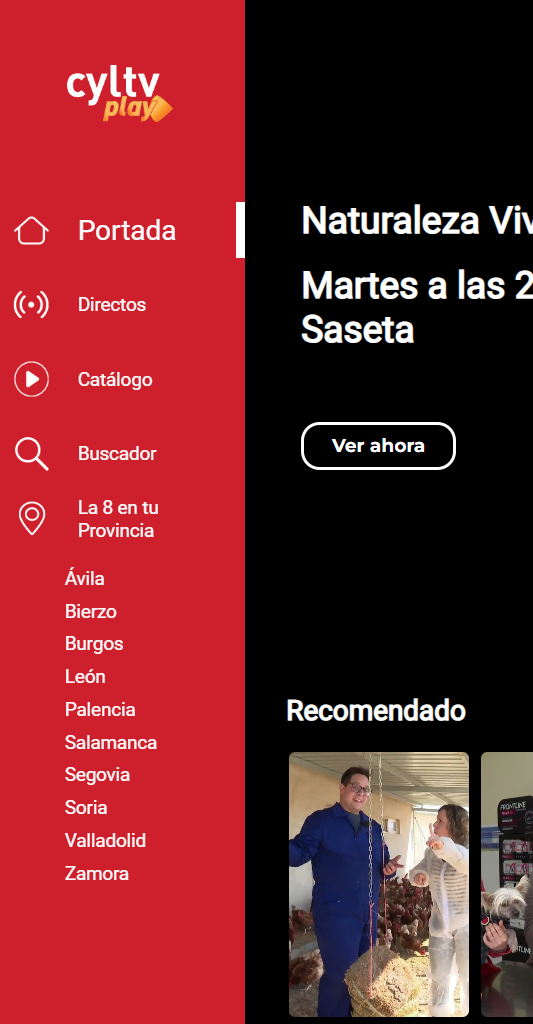
\includegraphics[width=\textwidth]{imaxes/OTT/menu_lateral_abierto.png}
        \subcaption{Menú lateral abierto}
        \label{fig:menu_lateral_abierto}
    \end{subfigure}
    \caption{Menú lateral}
\end{figure}

Durante el desarrollo del proyecto se probaron diferentes maneras de implementar el movimiento en la interfaz. Inicialmente, 
se comenzó moviendo los elementos hacia el foco y, más tarde, se decidió utilizar las funcionalidades de \textit{scroll} de HTML, 
que permite desplazar elementos sin realizar cálculos de posición. Sin embargo, ambas opciones fueron finalmente descartadas 
en favor de la utilización de las funcionalidades de \textit{transform} de CSS. Tras analizar las tres alternativas, 
se concluyó que el uso de \textit{transform} era prácticamente obligatorio. Aunque la opción de \textit{scroll} es más sencilla 
y presenta múltiples ventajas, su uso resulta menos eficiente, exigiendo un mayor esfuerzo al navegador. En el caso de 
ordenadores y dispositivos móviles, este esfuerzo no es tan significativo, pero en el caso de las televisiones, 
que cuentan con menos recursos, la aplicación se percibía lenta y pesada. La primera opción fue descartada porque es 
más efectivo y eficiente mover la pantalla completa en lugar de reordenar cada elemento por separado.

En futuras implementaciones, y con una optimización más avanzada de la aplicación, no se descarta estudiar nuevamente 
la funcionalidad de \textit{scroll} debido a sus ventajas. Sin embargo, por el momento, se seguirá utilizando la funcionalidad 
de \textit{transform} de CSS. Aunque el cambio no es urgente ni necesario, ya que para el usuario no supone una diferencia 
significativa en cuanto a la experiencia de uso, sí mejora el rendimiento general de la aplicación.

\subsubsection{Selección de un componente}
\label{sec:seleccion_componente}

Una vez que se ha movido el foco al elemento deseado, el siguiente paso es seleccionar dicho elemento. 
Para ello, cada componente tiene asociado un evento de selección que se activa al pulsar el botón de selección 
del mando a distancia. Este evento permite ejecutar la acción correspondiente al elemento seleccionado.

Las acciones desencadenadas por estos eventos pueden ser la creación de una nueva pantalla (cuando se selecciona 
una opción del menú lateral) o la creación de una pantalla de detalle (cuando se selecciona un contenido). 
En el caso de crear una nueva pantalla, se sigue el mismo proceso utilizado para la creación de la pantalla principal, 
mostrándose la nueva pantalla en la aplicación y almacenando la anterior en una pila de pantallas. 
Cuando se selecciona un contenido, se genera una pantalla de detalle con la información correspondiente 
al contenido seleccionado.


\subsubsection{Creación de la pantalla de detalle}
\label{sec:creacion_pantalla_detalle}
La pantalla de detalle muestra la información detallada de un contenido. Esta pantalla se genera en función de la información recibida 
tras realizar una llamada a la API con el identificador del contenido seleccionado.

Existen dos tipos de pantallas de detalle en función del tipo de contenido: contenedores y contenidos. Los \textbf{contenedores} son aquellos 
que agrupan otros contenidos, como una serie que contiene capítulos. Los \textbf{contenidos}, por su parte, son elementos finales, como una película, 
un capítulo o un partido, y no tienen elementos hijos asociados.

La pantalla de detalle de un contenedor incluye una ficha con la información del contenedor, una lista de los contenidos que agrupa y una 
lista de contenedores relacionados. El movimiento a través de los contenidos hijos se realiza de manera vertical, similar al funcionamiento 
en la pantalla principal, mientras que para los contenidos relacionados, se utiliza un movimiento horizontal, como en los widgets de la pantalla principal.

\begin{figure}[H]
    \begin{subfigure}[c]{0.5\textwidth}
        \includegraphics[width=\textwidth]{imaxes/OTT/pantalla_detalle_contenedor1.png}
        \subcaption{Pantalla de detalle de un contenedor}
        \label{fig:Widget_banner_contenedor}
    \end{subfigure}
    \hspace{0.1\textwidth}
    \begin{subfigure}[c]{0.5\textwidth}
        \includegraphics[width=\textwidth]{imaxes/OTT/pantalla_detalle_contenedor2.png}
        \subcaption{Pantalla de detalle de un contenedor}
        \label{fig:Widget_mosaico}
    \end{subfigure}
    \caption{Pantalla de detalle de un contenedor}
\end{figure}

Por otro lado, la pantalla de detalle de un contenido está compuesta por una ficha con la información del contenido. En esta ficha se incluye el título, 
el contenedor padre (si lo tiene, como en el caso de un capítulo de una serie, donde se muestra la serie a la que pertenece), una descripción corta, un 
botón que permite desplegar un popup con toda la información completa, los iconos de rating y edad, un botón de reproducción y, en caso de que la 
funcionalidad lo permita, un botón para añadir a favoritos. También se incluye una lista de contenidos relacionados.


\begin{figure}[H]
    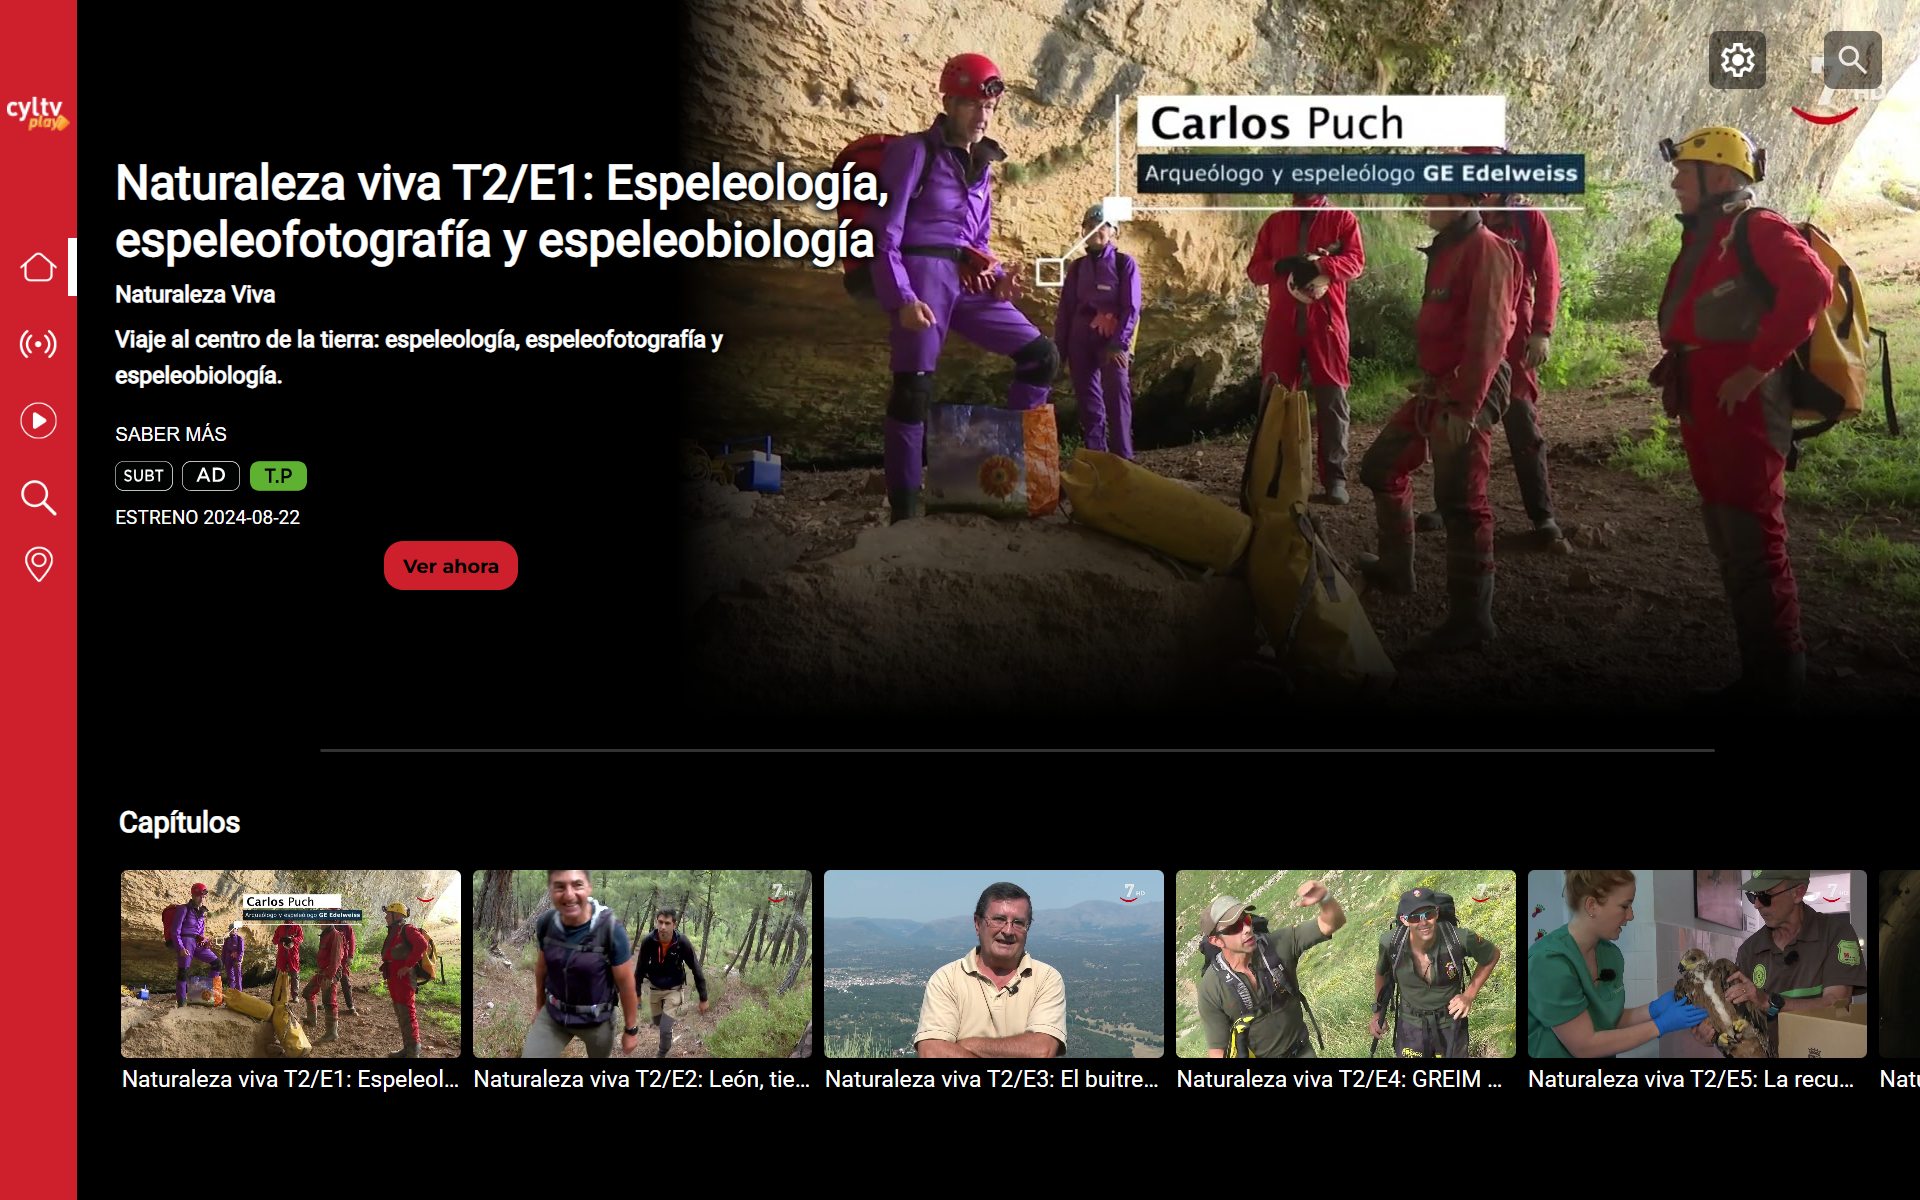
\includegraphics[width=0.4\textwidth]{imaxes/OTT/Pantalla_detalle_contenido.png}
    \caption{Pantalla de detalle}
\end{figure}

\subsubsection{Reproducción de un contenido}
\label{sec:reproduccion_contenido}

La reproducción de un contenido es una de las funcionalidades más importantes de la aplicación. Para acceder a ella hay dos opciones: a través de la pantalla de detalle 
del contenido explicada en el punto anterior, o si un contenido tiene el \textit{trigger} de reproducción activado, se podrá acceder a la reproducción directamente desde la pantalla 
principal. Al seleccionar el botón de reproducción, la aplicación obtiene la información del contenido. En esta información se comprueba si el contenido 
necesita autenticación para ser reproducido y, en caso afirmativo (el usuario ya debería estar logueado), se comprueba si el usuario tiene permisos para ver el contenido. 
Esta es una comprobación de seguridad, ya que en caso de no tener acceso al contenido, el botón de reproducción aparecerá deshabilitado. Si el usuario tiene acceso, 
se realizan varias comprobaciones:

\paragraph{Origen del contenido:} Lo primero es comprobar de dónde proviene el contenido. Existen dos opciones: que esté alojado en la base de datos de la empresa o 
en la del cliente. Si está en la del cliente, la URL del video ya estará en la información del contenido. En caso de estar en la base de datos de la empresa, se deben 
realizar una serie de comprobaciones para obtener la URL del video. Estas comprobaciones varían según si el contenido es gratuito o de pago; si es gratuito, la URL se puede 
construir directamente con la información disponible, pero si es de pago, se requieren verificaciones adicionales.

\paragraph{Reproductor:} No todos los dispositivos pueden utilizar el mismo reproductor. Los ordenadores son más permisivos en este aspecto, pero las televisiones no. En 
el caso de los ordenadores, incluso existe la opción de que la API devuelva un \textit{player} ya construido para ser usado directamente en la aplicación, aunque esta opción no 
se utiliza por el momento. El código detecta en qué sistema operativo (SO) y con qué tipo de contenido se está trabajando. Por el momento, hay dos reproductores disponibles 
(\textit{VideoJs} y \textit{ShakaPlayer}) y dos tipos de video (\textit{VoD} y \textit{Lives} o \textit{YouTube}). Para cada caso, se monta el reproductor de manera específica.

Una vez que el video se está reproduciendo, el usuario dispone de las funcionalidades básicas para controlar la reproducción: pausa, play, adelantar, retroceder y salir. 
Si la funcionalidad está permitida y el usuario está registrado, la aplicación guarda el instante en el que se detuvo la reproducción, permitiendo que se 
pueda continuar viendo el contenido desde el mismo punto en el que lo dejó.

\subsubsection{Añadir a favoritos}
\label{sec:anadir_favoritos}

En caso de permitir usuarios registrados, la aplicación ofrece la funcionalidad de añadir contenidos a favoritos. Para ello, en la pantalla de detalle de contenido 
se muestra un botón en forma de corazón, que permite agregar el contenido a la lista de favoritos. Si el contenido ya está añadido a favoritos, el botón aparece en 
color rojo, y pulsando sobre él se elimina de la lista de favoritos.

\subsubsection{Búsqueda de contenidos}
\label{sec:busqueda_contenidos}

La búsqueda de contenidos es una funcionalidad esencial de la aplicación. Se puede acceder a ella de dos formas: a través del menú lateral o mediante una opción situada 
en la parte superior derecha de todas las pantallas. Al abrir el menú de búsqueda, se muestra un campo de texto donde el usuario puede introducir el nombre completo o 
parcial del contenido que desea buscar. Al hacer clic en el botón de búsqueda, la aplicación realiza una llamada a la API con el nombre del contenido y recibe una lista 
de los contenidos que coinciden con el criterio de búsqueda. Esta lista se presenta en una pantalla de resultados en formato de mosaico.

\subsubsection{Obtención de la información de un directo}
\label{sec:obtencion_informacion_directo}

La obtención de la información de un directo permite a la aplicación recibir datos en tiempo real de los contenidos en emisión. Para ello, se realiza una llamada a la API 
con el identificador del directo, obteniendo la información a través de un EPG (Electronic Program Guide). Este EPG es un archivo JSON que contiene la información de los 
contenidos que se emitirán en un periodo determinado. La aplicación analiza este JSON y extrae la información en tiempo real del directo, incluyendo el título del contenido 
y su progreso, el cual se calcula a partir de los tiempos de inicio y fin del contenido marcados en el JSON, mostrando dicha información en la barra de progreso.
